\chapter{Introduction}\label{C:intro}
Everyone experiences the process of making decisions during his life. As a matter of fact, drastically the life of an individual can be synthesized in its \textit{perception} of the world and its \textit{interaction} with it. The concepts of perception and interaction may seem quite straightforward to understand: for a human the perception of the world comes from its senses and the interaction comes from its possibility to change its surroundings. On the contrary, these concepts are actually absolutely hard to define and aroused, over the centuries, a strong debate between scientists, biologists, and even philosophers.

\section{Perception and interaction}
We assume that, by definition, an individual perceives the surrounding and acts on it in order to achieve the \textit{goals} expressed by its will. In other words, all the actions performed by an individual are made to satisfy its will to obtain something from the world it lives in. This task is naturally carried out by humans, but implies some challenging problems that are hard, or unfeasible, to solved. One of these derives from the intrinsic \textit{uncertainty} of the perception we have of the world around us. Indeed, the perception of the world consists in the interpretation of the information provided by the senses, but the process of information retrieval by the senses and the mental processes to understand them, inevitably introduce a certain level of noise that distorts the true original information. On the other hand, interaction with the world deals with the individual's willingness to perform actions to change the surrounding, but this apparently simple operation involves complex biological mechanisms to coordinate the body according to the will and difficulties in the perception of the consequences of the interaction. Moreover, the concept of goal can be unclear and the individual may result in performing actions without being sure of what it wants.
It is arguable that discussing about the concept of true information and the concept of will requires strong theoretical considerations since they are both hard to define concepts. For many centuries, scientists and philosophers debated about these topics, in particular trying to solve complex problems like the real nature of perceivable things and the concept of free will. However, to make the discussion of these concepts suitable for our purposes throughout this thesis, we lighten their definition to the one provided by common sense.

\section{Learn how to act with Reinforcement Learning}
\gls{rl}~\cite{sutton1998reinforcement} is a subfield of \gls{ml} that aims to realize autonomous \textit{agents} able to learn how to act in a certain \textit{environment} in order to maximize an objective function; this is achieved by providing the agent with the perception of its \textit{state} in the environment and making it learn the appropriate \textit{action} to be performed, where an action can be seen as an atomic operation that brings the agent from one state to another. The objective function represents a measure of how well the agent is accomplishing its task in the environment and is usually formalized by a discounted sum of \textit{rewards} obtained after each action (Figure~\ref{F:rl}). The sum is discounted to give more importance to the most recent rewards w.r.t. the ones further in the future. The reward function, i.e. the function returning the reward after each action, is not a concrete part of the environment, but it is often designed by a human who decides whether a certain behavior must be reinforced by (returning a positive reward) or inhibited (returning a negative reward).

\begin{figure}[t]
\begin{minipage}{\textwidth}
\begin{center}
  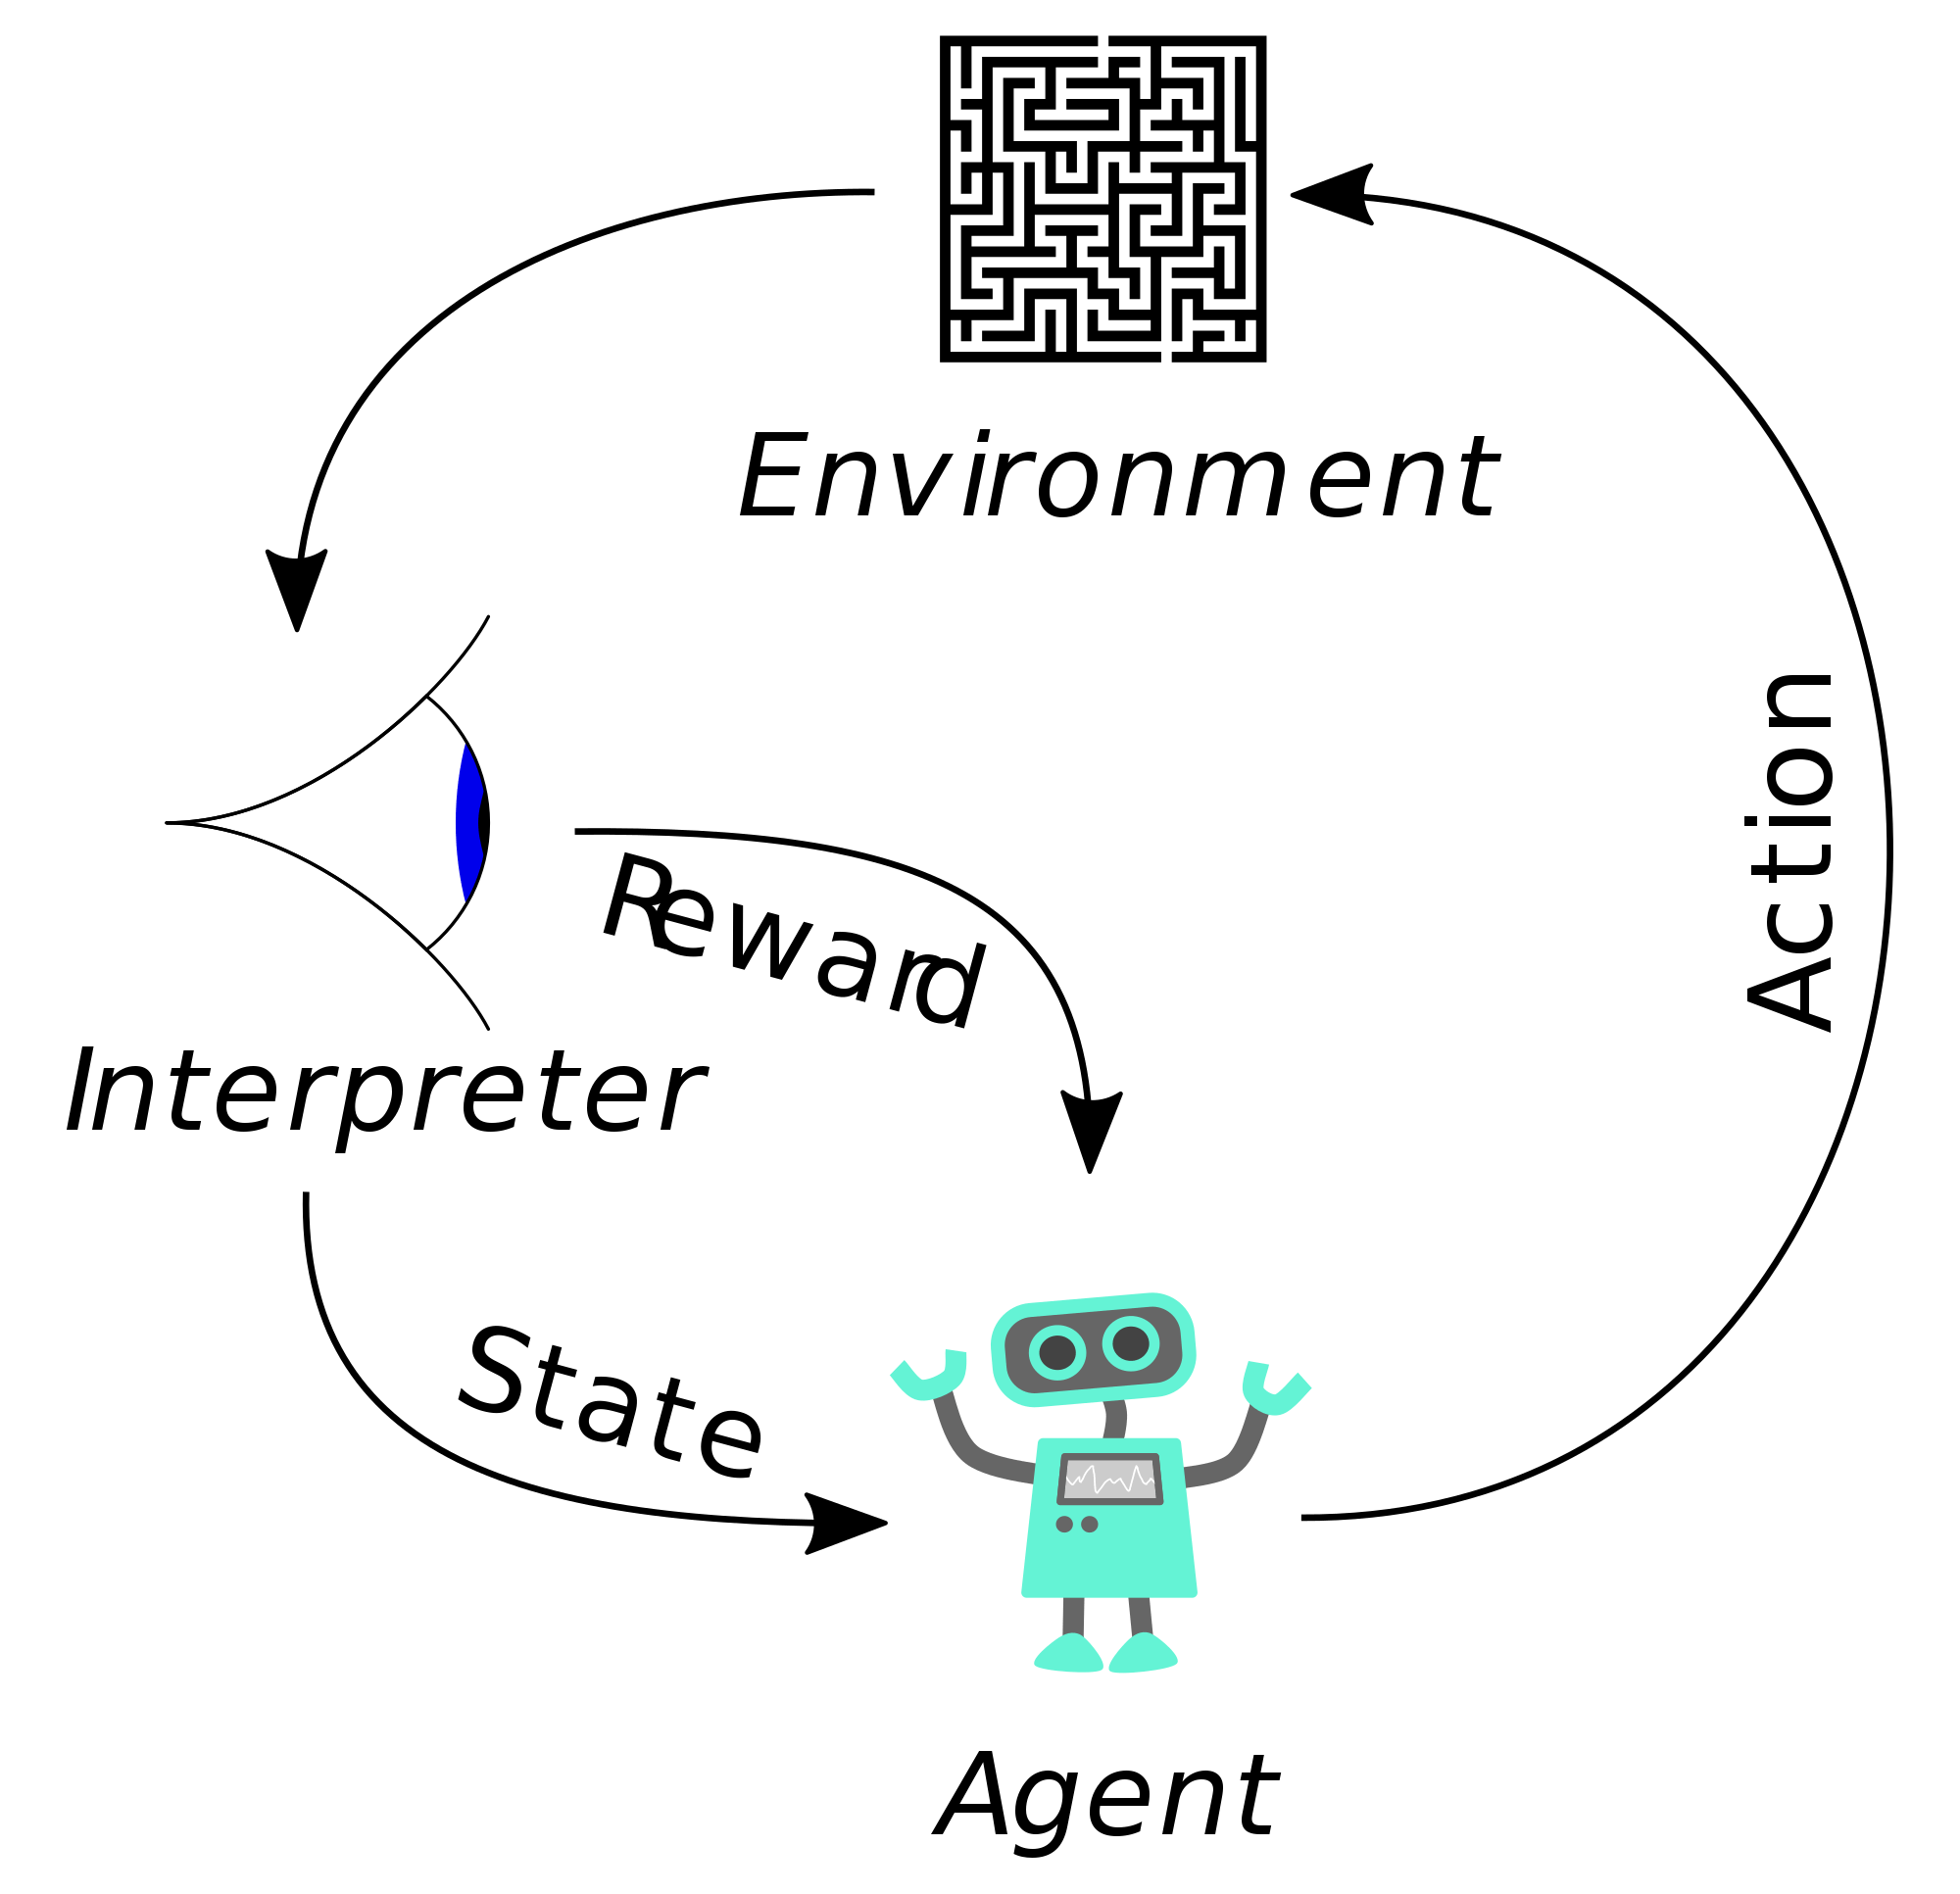
\includegraphics[scale=.1]{img/rl.png}
\end{center}
\end{minipage}
\caption[Reinforcement Learning problem scheme]{The scheme of a Reinforcement Learning model.}\label{F:rl}
\end{figure}

\subsection{Uncertainty in Reinforcement Learning}
The major challenge of \gls{rl} is represented by uncertainty. In fact, initially, the agent is not provided with the knowledge of how the environment will react to its actions, thus it does not know whether an action would be good or not to maximize its objective function. In other words, before trying an action, it does not know if that action will get a positive or a negative reward, and it does not know if that action will let it go to the expected state or not. Thus, the former problem can be seen as uncertainty in the reward function and the latter as uncertainty in the transition (i.e. model) function. In some cases, also the uncertainty in the perception of the current state of the agent is considered, making the problem more complex.

The uncertainty issue results in the need of the agent to try actions in order to improve its knowledge of the environment. This process delays the collection of high rewards, but helps the agent to reduce its uncertainty. However, since the objective function is a sum of discounted rewards where later rewards worth less than recent ones, the agent also needs to learn fast in order to learn to perform the most rewarding actions as soon as possible. The need to \textit{explore} to reduce uncertainty and the need to \textit{exploit} the actions believed to be good introduces an important problem known as \textit{exploration-exploitation dilemma}.

\subsection{Balancing exploration and exploitation}
The exploration-exploitation dilemma has been broadly studied in the \gls{mab} field, a particular case of the \gls{rl} problem with a single state~\cite{lai1985asymptotically}. In this problem, the goal is to find the sequence of optimal actions minimizing the choice of suboptimal ones, i.e. the sequence of actions that allows to maximize the return. The simplistic setting of the \gls{mab} problem allows to theoretically study the balancing of exploratory and exploitative actions, for instance, to derive upper confidence bounds on the \textit{regret}, i.e. a measure of the return lost in performing non-optimal actions~\cite{bubeck2012regret, agrawal2012analysis, vermorel2005multi}, and several algorithms to address this problem have been proposed such as UCB1~\cite{auer2002finite} and Thompson Sampling~\cite{thompson1933likelihood}.

The \gls{rl} setting complicates the \gls{mab} problem because of the presence of multiple states and of the fact that the sequence of visited states strictly depends on the chosen actions. This makes the exploration-exploitation dilemma less tractable in terms of computational and complexity feasibility. Indeed, the quality of the actions must now be evaluated for each state, contrary to the \gls{mab} case where the presence of a single state simplifies the problem. This issue is what makes \gls{rl} so challenging and has been addressed for decades in the literature.

\section{My research}
The strong connection between uncertainty and the exploration-exploitation dilemma is highlighted by the previous considerations and it is intuitive how the effectiveness of an \gls{rl} algorithm depends on its ability to reduce the uncertainty of the agent in a computational and data-efficient way. The \gls{rl} literature contains many algorithms and methodologies proposed to make the agent learn a good policy by aiming at efficiency; however, despite addressing the reduction of uncertainty through experience, only a few of them explicitly model the uncertainty to learn.

\subsection{What is my research about}
During my Ph.D., we studied ways to develop algorithms that exploit uncertainty since the explicit consideration of it has been shown to be often useful for improving the performance and efficiency of learning. One of the most common techniques to explore is known as $\varepsilon$-greedy and consists in performing, at each state, a random action with probability $\varepsilon$ and the action considered the best with probability $1 - \varepsilon$. This exploratory policy does not consider the uncertainty of the agent and simply randomly collects samples with the drawback of requiring a huge amount of experience to learn effective policies. This is shown especially in recent works in the field of \gls{drl}~\cite{mnih2015human, van2016deep, wang2015dueling} which studies the application of \gls{dl}~\cite{lecun2015deep} models and methodologies to exploit their strong ability to generalize with the purpose to solve complex problems that were unfeasible before. The research on \gls{drl} brought to the realization of groundbreaking works in which the authors were able to reach the state of the art in extremely complex games such as Go~\cite{silver2016mastering, silver2017mastering} and chess~\cite{silver2017chess}.
However, the extraordinariness of these results is comparable to the amount of experience required by these algorithms to work. For instance, in~\cite{mnih2015human} the experiments are performed using $50$ millions of samples corresponding to three days of computation and several weeks of human play; obviously this huge demand of time and computational power could make the execution of the algorithm impractical in some cases.

In addition to the exploration problem, we studied the problem of \textit{estimating maximum action-values} in value-based \gls{rl}. This latter problem is historically known in literature and is a critical issue in many value-based algorithms that may seriously affect the performance, as shown in recent works~\cite{smith2006optimizer}. In particular, a well-known problem consists in the overestimation of the maximum action-values leading to poor empirical results in certain type of problems. To solve this, some recent works~\cite{van2010double, xu2013mab, van2015deep} proposed a new estimator that provides an underestimation instead of an overestimation, which is helpful in problems where the overestimation leads to bad results.

\subsection{What we have done}
We worked on the problems of exploration and maximum action-value estimation with the purpose to work out some new effective techniques. In particular, for the former problem, we developed two new exploration strategies based on the concept of Optimism in the Face of Uncertainty, a principle that exploits uncertainty to visit mostly unknown states in an environment. On the other hand, for the latter problem we worked on the proposal of a new maximum action-values estimator that computes an estimate of the maximum action-values basing on uncertainty. This estimate can both be positively and negatively biased, a property that helps to obtain good results in heterogeneous problems.

My Ph.D. research led to the publication of four conference papers, most of which focused on the previously described topic. We also developed, together with a colleague of mine, an \gls{rl} Python library called \textit{Mushroom} which had the initial purpose of facilitating my research, but which has become larger and larger allowing now to do \gls{rl} research for general purposes. Details about Mushroom are reported in Appendix~\ref{App:msh}. Other works presented here are still ongoing and/or under review.

\subsection{Outline of the thesis}
The whole document is divided in four parts, with this introduction included in the first one:
\begin{itemize}
 \item the \textbf{introductory} part includes this chapter and Chapter~\ref{C:soa} which introduces the main concepts of \gls{rl} starting from the fundamental theory and then giving a description of several methodologies related to this thesis in order to provide a general, but useful, overview of what is necessary to understand the following chapters;
 \item the \textbf{Bellman update} part includes the description of three publications I made on ways to exploit the uncertainty in the context of value-based \gls{rl} and more specifically in the famous algorithm of $Q$-Learning. In particular, Chapter~\ref{C:mev} describes a novel way of addressing the problem of overestimating the Maximum Expected Value in $Q$-Learning and Chapter~\ref{C:rq} describes a novel way of dealing with uncertainty in the estimation of the Bellman operator components;
 \item the \textbf{Uncertainty-Driven Exploration} part includes two works about the exploitation of uncertainty to drive exploration. Chapter~\ref{C:ts} describes a set of algorithms for estimating uncertainty of action-values to allow the use of an exploration policy inspired by Thompson Sampling. Chapter~\ref{C:opt} introduces a variant of the Bellman operator that incorporates an optimistic update of the action-value estimate in order to favor exploration according to the principle of Optimism in the Face of Uncertainty;
 \item the \textbf{conclusive} and last part concludes the thesis by resuming the previous chapters and giving my considerations about the research I have done and on what I think will be interesting to pursue in the following years, by me or someone else!
\end{itemize}
